%Experimental Methodology – in this section, you should describe the environment where you did the experiments, tools you used (compilers, libraries, profilers, simulators) and benchmarks that you used. Here you should tell what is your evaluation criteria (e.g. Speedup) and metrics (e.g. throughput). Anything important that was made to conduct the experiments should be here (e.g. preparing traces for reproducing deterministic executions). If your experimental methodology has limitations you should mention them here (e.g. when using simulator you used small data input sets).

\section{Simulations}
\label{sec:simulations} 

\subsection*{Introduction} 
In this section, we describe all simulations which we performed in our work. We start with definition of our evaluation metrics in Section~\ref{sec:sim-evaluation} and te we give a short description of datasets used for our simulations in Section~\ref{sec:sim-data}. The main part are the descriptions of used modified versions of BAL in Section~\ref{sec:sim-our}. Finally, we end with additional experiments used to prove or disprove our hypotheses in Section~\ref{sec:sim-exp}.


\subsection{Evaluation methods} 
\label{sec:sim-evaluation} 

Following~\citet{farkas2013bal}, we measured two key properties of a BAL-like network. The more important being \emph{success rate} and second being \emph{convergence time}. 

\paragraph{Success rate.}  
Before comparing \emph{given} outputs on both visible layers the activations $Y^F$ and $X^B$ are classified by a treshold: 
\begin{equation} 
  g_k =
  \left\{
	  \begin{array}{ll}
		  1 & \mbox{if } x_k^B > 0.5 \\
		  0 & \mbox{otherwise}
	  \end{array}
  \right.  
\end{equation} 
By having a set of given vectors $G^I$ and the target vectors $T^I$ for inputs $I \in \mathbb{S}$, we distinguish two main success measures: 

%TODO remove itemize
\begin{itemize}
  \item \emph{Bit success (bitSucc)} defined as $bitSucc = avg_{I \in \mathbb{S}} \sum_i |T_i^I - G^I_i|$ and 
  \item \emph{Pattern success (patSucc)} defined as 
    \begin{equation}
      patSucc = avg_{I \in \mathbb{S}} \left\{
	      \begin{array}{ll}
		      1 & \mbox{if } T^I = G^I \\
		      0 & \mbox{otherwise}
	      \end{array}
      \right.
    \end{equation} 
\end{itemize} 

\paragraph{Convergence time.} The are several possibilities when to stop the learning algorithm. \emph{Converge time} is the number of epochs before the stop. Usually, training could be stopped for two reasons. The network could either reach the \emph{stopping criteria} or the maximum epoch is reached. Given by nature of used datasets we trained the neural networks while $patSucc^F \neq 1$. In case of the \emph{digits}~(\ref{sec:datasets-digits}) dataset we decided to stop the training if $patSucc^F$ was not increased for 3 epochs. Note that we are motivated to decrease the convergence time as it makes the training process faster.  
 


\subsection{Datasets}  
\label{sec:sim-data} 

For analysing our versions of BAL~(\ref{sec:models-bal}) we have chosen three datasets on which we tested and compared the performance of our models. 

\subsubsection{4-2-4 Encoder} 
\label{sec:datasets-auto4}


The \emph{4-2-4 econder} task is the simplest dataset we have been working with. It consists of four four--dimensional samples $(1,0,0,0)$, $(0,1,0,0)$, $(0,0,1,0)$ and $(0,0,0,1)$ which are each mapped to itself. We use two units on the hidden layer what gives us the 4-2-4 architecture. The 4-2-4 encoder task is a well--known problem and used previously for testing GeneRec~\citep{o1996bio} and BAL~\citep{farkas2013bal}. In the case of BAL only 60--65\% \emph{patSucc} was achieved which leaves room for improvement. Also this dataset as it~is convenient for testing novel approaches as the learning progress of the network could be checked by hand and eye. 

\subsubsection{Complex binary vector associations} 
\label{sec:datasets-k3}

The \emph{complex binary vector associations (CBVA)} task was used in~\citet{farkas2013bal} and its motivated by the sensory--motor mappings between distributed patterns~\citep{farkas2013bal}. The task is to associate sixteen 16--dimensional vectors all with 3 active units. There are always 4 distinct overlapping input patterns associated with exactly one output pattern. As the association is not unique in the \emph{backward} way it~is impossible to achieve perfect $bitSucc^B$ or $patSucc^B$. Therefore, we would expect from the network to give a \emph{blend} of the four input patterns corresponding to one output. 

\begin{figure}[H]
  \centering
  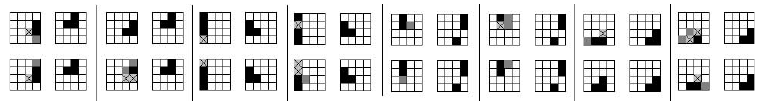
\includegraphics[width=0.98\textwidth]{img/datasets-k3.png} 
  \caption{BAL performance on \emph{CBVA}. Black color stands for target--estimate match, gray for target only and gray with a cross for false--positive estimate~\citep{farkas2013bal}.}
  \label{fig:datasets-k3}
\end{figure}

%tail -n +2 train.csv | sed 's/,/ /g' | awk 'BEGIN{FS=" "}{for(i=2;i<=NF;i++) {printf "%f ", $i / 256.0} printf "\n"}' >> buf.in
%echo "38000 784" > digits.in
%echo "4000 784" > digits.test.in
%tail -n +2 train.csv | sed 's/,/ /g' | awk 'BEGIN{FS=" "}{for(i=0;i<=9;i++) printf("%d ", $1 == i ? 1 : 0); printf "\n"}' > buf.out
%echo "38000 10" > digits.out
%echo "4000 10" > digits.test.out
%head -38000 buf.in >> digits.in 
%tail -4000 buf.in >> digits.test.in 
%head -38000 buf.out >> digits.out
%tail -4000 buf.out >> digits.test.out
%rm buf.* 
\subsubsection{Handwritten digits} 
\label{sec:datasets-digits} 

The well--known MNIST dataset of \emph{handwritten digits}~\citep{digits2014mnist} first analysed by~\citet{lecun1998gradient} consists of 42,000 $28 \times 28$ grayscale images mapped to ten classes each representing one digit. We have chosen this dataset for three reasons. First, it~is big and complex enough to test the practicallity of our models. Second, performance of many models is known on this dataset and therefore, we can easily compare performance of our models to these models. And third, we can easily visualize the backward \emph{blend} representations and intuitively see if our models perform well. These visualisations could be found in Section~\ref{sec:our-backward-repre}. 

\begin{figure}[H]
  \centering
  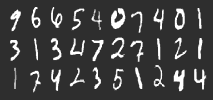
\includegraphics[width=0.4\textwidth]{img/digits.png} 
  \caption{Samples from the \emph{digits} dataset.}
  \label{fig:datasets-digits}
\end{figure}




\subsection{Models}

\subsubsection*{Introduction} 
TODO rewrite  
In this section we describe our versions of BAL for which we ran experiments. We examined several common neural network modifications such as adding \emph{momentum} or learning in \emph{batch mode}. We also examined novel approaches to our knowledge such. In general onle few variants of the original BAL model were successful as we will see in the following chapter. 

%We ignored existing models which are trained non-locally such as: 
%\begin{itemize} 
%\item Training feedforward networks with the Marquardt algorithm
%\item Extreme learning machine: a new learning scheme of feedforward neural networks
%\end{itemize} 
%Although the learning speed could be significantly better compared to traditional BP or our BAL. 


\subsubsection{Two learning speeds} 
TODO reformulate. 
In this model we use two learning speeds. First, $\lambda_I$ for weights $W_{IH}$ and $W_{OH}$ and second, $\lambda_H$ for weights $W_{HI}$ and $W_{HO}$. Both $\lambda_I$ and $\lambda_H$ are constant for the whole learning phase and therefore this model is consistent with our bio-plausibility assumptions. 

Our simulations show that setting $\lambda_I << \lambda_H$ could lead to significantly better performance in comparison to the standard BAL model. 

Our intuitive explanation behind is that $h^F - h^B$ converges to zero slower and therefore error terms $(o - t)$ and $(i - s)$ could impact $W_{IH}$ and $W_{OH}$ for more epochs. Moreover we can explain this model in terms of bio-plausibility. The perception of input to internal representation is changed only little over time and only the reconstruction to target pattern from internal representation is trained hard. 

TODO make sure this idea is novel enough (haven't found so far) \\
TODO try it also with CHL and GeneRec.  \\ 
 

\subsubsection{Recirculation BAL} 
\label{sec:our-bal-recirc} 

%\paragraph{Introduction} %====================
The aim of \emph{Recirculation BAL} is to combine the ideas of BAL~(\ref{sec:models-bal}) and iterative activation from GeneRec~(\ref{sec:models-generec-activation}). In other words, instead of computing the forward pass using only $W^{IH}$ and $W^{HO}$ we add a recirculation step between matrices $W^{HO}$ and $W^{OH}$, and similary for the backward pass and $W^{HI}$ and $W^{IH}$. We tried two approaches of such a combination. The first one is \emph{Bidirectional Iterative Activation (BIA)} \label{sec:our-bia} which is a straightforward implementation of the idea. Activation computation of BIA is shown in Table~\ref{tab:our-bia-activation}.  

\begin{table}[H] 
  \centering
  \begin{tabular}{|cccl|}
    \hline
    Layer & Phase & Net Input & Activation\\
    \hline
    \Bx & F & - & $x^{\rm F}_i$ = stimulus\\ [1ex]
    \Bh & F & \hspace{0.3cm}$\eta^{\rm F}_j = \sum_i w_{ij}^{IH}x^{F}_i + \sum_k w_{kj}^{OH}y^{F}_k$\hspace{0.3cm} & $h^{\rm F}_j = \sigma(\eta^{\rm F}_j)$\hspace{0.3cm}\\ [1ex]
    \By & F & $\eta^{\rm F}_k = \sum_j w_{jk}^{HO}h^{F}_j$ & $y^{\rm F}_k = \sigma(\eta^{\rm F}_k)$\\ [1ex]
    \hline
    \By & B & - & $y^{\rm B}_k$ = stimulus\\ [1ex]
    \Bh & B & $\eta^{\rm B}_j = \sum_k w_{kj}^{OH}y^{\rm B}_k + \sum_i w_{ij}^{IH}x^{\rm B}_i$ & $h^{\rm B}_j = \sigma(\eta^{\rm B}_j)$\\ [1ex]
    \Bx & B  & $\eta^{\rm B}_i = \sum_j w_{ji}^{HI}h^{\rm B}_j$ & $x^{\rm B}_i = \sigma(\eta^{\rm B}_i)$\\
    \hline
  \end{tabular}
  \caption{Activation for BIA~(\ref{sec:our-bia}). The only difference with BAL~(\ref{tab:models-bal-activation}) are the recurrent terms $\sum_k w_{kj}^{OH}y^{F}_k$ and $\sum_i w_{ij}^{IH}x^{\rm B}_i$.}
  \label{tab:our-bia-activation}
\end{table} 

The second one is \emph{Bidirectional GeneRec (BiGeneRec)} \label{sec:our-bigenerec} which has three phases. The first $F^{-}$ phase is same as the \emph{minus} phase of GeneRec and the third $C^{+}$ phase is same as the \emph{plus} phase of GeneRec. The second $B^{-}$ phase is same as the $F^{-}$ phase but from back to front. In other words we can treat $F^{-}$ and $B^{-}$ phases as \emph{forward} and \emph{backward} minus phase of GeneRec and the $C^{+}$ phase as the plus phase of GeneRec. As in the $F^{-}$ phase, only the forward weights $W^{IH}$ and $W^{HO}$ are updated and in the $B^{-}$ phase only the backward weights $W^{OH}$ and $W^{HI}$ are updated. We can treat weight updates of BiGeneRec as two independent GeneRec update steps. 

\begin{table}[H] 
  \centering
  \begin{tabular}{|cccl|}
    \hline
    Layer & Phase & Net Input & Activation\\
    \hline
    Hidden (h)   &  $C^{+}$  & $\eta^{+}_j = \sum_{i}w_{ij}^{IH}x^{\rm F}_i$ + $\sum_k w_{kj}^{OH}y^{\rm B}_k$ & $h^{+}_{j} = \sigma(\eta^{+}_j)$ \\
    \hline
  \end{tabular}
  \caption{Difference between BiGeneRec (\ref{sec:our-bigenerec}) and BIA (\ref{tab:our-bia-activation}) is the additional $C^{+}$ phase corresponding to the plus phase of GeneRec~(\ref{sec:models-generec}).} 
  \label{tab:our-bigenerec-activation}
\end{table} 

For both BIA and BiGeneRec we experimented with both asymmetric and symmetric versions. For the asymmetric version we experienced problems with \emph{fluctuation}. This is briefly discussed in Section~\ref{sec:generec-fluctuation} and in Section~\ref{sec:our-fluctuation}.  



\subsubsection{Candidate selection} 
\label{sec:our-candidates} 

\paragraph{Introduction.} 
The \emph{candidate selection} model was used to test and prove if some particular network \emph{features} \ref{sec:our-candidates-features} have an impact to the overall network performance. Only difference between standard BAL \ref{sec:models-bal} is that before the training phase $N$ networks are randomly generated from which a \emph{best candidate network} is selected based on \emph{feature function} defined as $F: \mbox{network} \mapsto \mathbb{R}$. The feature function was trained on a \emph{feature dataset} containing inficidual features and a binary label \emph{success}. The dataset was generated by running standard BAL, measuring features before the run and adding the success label after the training. The notion of most important features was used to design other models which reinforced these features, e.g. the \emph{Two learning rate} model \ref{sec:our-two-lambdas} for the \emph{h\_f\_b\_b\_dist} feature. 

\begin{figure}[H]
    \begin{lstlisting} 
      candidates = [generate_network for i in range(0, N)] 
      candidate = max(pair(fitness(c),c) for c in candidates) 
      train(candidate.c) 
    \end{lstlisting} 
  \caption{Candidate selection pseudocode.}
  \label{fig:our-candidates-pseudocode} 
\end{figure} 

\paragraph{Features.}
\label{sec:our-candidates-features}

TODO describe it more \\
TODO note when auto / hetero associative \\

We denote $X_I$, $H_I$ and $Y_I$ as the front, hidden and back activation \emph{vector}s for input $I$ (and the corresponding target). For the rest of the notation please consult \ref{tab:models-bal-activation}. We measured the following \emph{features}: 
\begin{itemize} 
\item h\_dist - $avg_{I \neq J}\left(dist(H_I^{+},H_J^{+})\right)$.
\item h\_f\_b\_dist - $avg_{I}\left(dist(H_I^{-},H_I^{+})\right)$.
\item	v\_f\_b\_dist - as h\_f\_b\_dist but for visible layer: $avg_{I}\left(dist(Y_I^{-},X_I^{+})\right)$. 
\item matrix\_w - average weight of matrices $W^{IH}$, $W^{HO}$, $W^{OH}$ and $W^{HI}$. 
\item matrix\_sim - sum of $|a_{ij} - b_{ij}|$ per pairs $(a,b) \in ((W^{IH}, W^{OH}),\, (W^{HI}, W^{HO}))$. 
\item \label{sec:our-in-triangle} in\_triangle - for hidden size equal two: check if hidden representations of inputs form a convex polygon, i.e.~if the hidden representations are lineary separable \ref{sec:models-perceptron}. 
\item fluctuation - when treating the opposing weight matrices, i.e.~$w_IH$ to $w_HI$ and $w_HO$ to $w_OH$, as in GeneRec activation computation \ref{eq:models-generec-activation} then \emph{fluctuation} measures:
\begin{equation}
  \label{eq:our-fluctuation}
  max_{I}\left(
    max_{i \in \mbox{\tiny units}}\left(
      |a_i(t_{\mbox{\tiny stop}}) - a_i(t_{\mbox{\tiny stop}-1})
    \right)|
  \right). 
\end{equation}

%\item err - current bit error 
%\item first\_second - sum of ratio of $(a_1, a_2)$ where $a_i$ is the $i$-th biggest output 
%\item sigma $\sigma$ - initial weight distribution 
%\item lambda $\lambda$ or $\lambda_h$ - common learning rate or learning rate for $W^{IH}$ and $W^{OH}$. 
%\item lambda\_h $\lambda_v$ - in the Two learning rate model \ref{sec:our-two-lambdas} the value of learning rate for $W^{IH}$ and $W^{OH}$
%\item momentum $\mu$ - \ref{sec:our-momentum}

%\label{sec:sim-evaluation-methods} 

%	//public static  int MEASURE_NOISE_SPAN = 9; 
%	//public static  int MEASURE_MULTIPLY_WEIGHTS = 9; 
\end{itemize} 

Also all \emph{parameters} of neural network were included such as $\lambda$, $\lambda_h$, $\lambda_v$ \ref{sec:our-two-lambdas}, momentum $\mu$ \ref{sec:our-momentum} and weight distribution $\sigma$ \ref{sec:our-sigma}. 


\paragraph{Results.} 
The following figure shows that when selecting the candidate with the highest \emph{h\_dist} among 100 randomly generated networks it could lead to about 10\% success increase. 

TODO Figure candidate selection compare to standard BAL (pdf) 

TODO Hidden distance (over 70\%); in triangle (68.3 \%). 

TODO Linear regression model. 
 
  

\subsubsection{Long training} 
even after 800,000 epochs there are some networks for which the error change
 

\subsubsection{Other}
TODO introduction (brief, experiment settings) 

%==========================================================
\paragraph{Momentum}
\label{sec:our-momentum}

\citep{rumelhart1986learning, yu1997efficient} is an extension for any learning rule of form $\Delta w_{ij}(t) = L(i,j,t)$ by adding a \emph{momentum} term: 
\begin{equation} 
  \Delta w_{ij}(t) = L(i,j,t) + \mu \Delta w_{ij}(t-1).
\end{equation} 
It is argued that momentum could overcome settling in local minima by using the second derivate (TODO cite). 

%==========================================================
\paragraph{Batch mode} learning method changes how the weight update rule is applied. Instead of updateing weights after each training sample, weight changes are accumulated for the whole epoch, i.e.~summing all weight changes for each sample, and weights are updated in \emph{batch} (TODO citation). One can observe that shuffling of samples has no effect at all. Therefore after the weights are initialized the learning algorithm becomes deterministic.

%==========================================================
\paragraph{Different learning rules.}
\label{sec:our-learning-rules}

Both for BAL \ref{sec:models-bal} and GeneRec \ref{sec:models-generec} is possible to try different learning rules mentioned in \ref{sec:models-generec-modifications}. We will denote such models as \emph{BAL-sym} and \emph{GR-sym} for symmetry perserving rule~\ref{eq:models-generec-learning-rule-sym}; \emph{BAL-mid} and \emph{GR-mid} for midpoint rule~\ref{eq:models-generec-learning-rule-mid} and \emph{BAL-chl} and \emph{GR-chl} for CHL rule~\ref{eq:models-generec-learning-rule-chl}. 

TODO not working with BAL -> analyse (GeneRec kind of ok) 

%==========================================================
\paragraph{Rerun} was designed to test if shuffling of samples has effect to network performance. First, $N$ networks are created with random weights~\ref{sec:our-sigma} with same parameters then are saved and trained. Second, the networks are loaded and each network is re--trained $k$-times. At the end difference between performance of the $k$ networks and the original network is measured. In this way it could be decided if the network performance depended on the shuffling of the training samples or on other network parameters. 

TODO rerun experiment (it has suspicious results) 

\begin{lstlisting}
All bad: 
err sigma lambda momentum success sample_ratio
0.0 2.3 0.7 0.0 19.296918767507005 6889/35700
1.0 2.3 0.7 0.0 68.05602240896359 24296/35700
2.0 2.3 0.7 0.0 12.644257703081232 4514/35700
3.0 2.3 0.7 0.0 0.0028011204481792717 1/35700

All good: 
err sigma lambda momentum success sample_ratio
0.0 2.3 0.7 0.0 99.98911353032659 64293/64300
1.0 2.3 0.7 0.0 0.01088646967340591 7/64300
//TODO overit ci dobre rozdelilo good / bad
\end{lstlisting}

We see that the networks which were successfull in the first run remained successfull in the re--runs. On the other side of the unsuccessfull networks changed their performance after re--run. 

%==========================================================
\paragraph{Hidden activations.}
\label{sec:our-hidden-activation} 

We observed that hidden activations tend to settle fast \ref{sec:our-candidates}, i.e. the weight changes become close to zero because $|H^F - H^B| \approx \overrightarrow{0}$. Therefore the network is de--facto reduced to a two--layer network between the constant hidden activations and the target values. Thus \emph{at least} all cases when the hidden activations are not linearly separable it is impossible for $w_{HI}$ and $w_{HO}$ to learn targets. This behaviour is demonstrated by the \emph{in\_triangle} measure \ref{sec:our-in-triangle}. 

A more formal explaination why the hidden activations tend to settle fast could be given by the GeneRec learning rule \ref{eq:models-generec-learning-rule}: 
\begin{equation} 
  \Delta w_{ij} = a_i(b_j - a_j),
\end{equation} 
which for the $W^{IH}$ and $W^{OH}$ yields: 
\begin{equation} 
  \Delta w_{ij}^{IH} = x^F_i(h^B_j - h^F_j) \\ 
  \Delta w_{ij}^{OH} = y^B_i(h^F_j - h^B_j). 
\end{equation} 
We see that both terms $(h^B_j - h^F_j)$ and $(h^F_j - h^B_j)$ push $W^{IH}$ and $W^{OH}$ in a way that $h^B_j = h^F_j$. This experiment was the main reason to start experimenting with the Two learning rate model \ref{sec:our-two-lambdas}. 

%==========================================================
\paragraph{Dynamic weight lambda.} 
\label{our-dynamic-lambda} 
The idea of \emph{dynamic weight lambda} (TODO cite) is to have separate learning rate for each weight: 
\begin{equation}
\Delta w_{ij}(t) = \lambda_{ij}(t) a_i\left(b_j - a_j\right), 
\end{equation}
%where $b_j(t-1) - a_j(t-1)$ is the error term and $\lambda_{ij}^{t-1}$ is the learning rate from the last epoch. 
There are several approaches how to set $\lambda_{ij}(t)$. Dynamic lambda per weight \emph{delta--bar--delta--rule} \citep{jacobs1988increased} (TODO parse and link). \\
Adaptive lambda \citep{riedmiller1993direct} \\
Dynamic lambda \citep{yu1997efficient} \\ 
TODO more simulations.  \\
TODO citations.  \\
This model was inspiration for the two lambda model \ref{sec:our-two-lambdas}. 

%==========================================================
\paragraph{Symmetric BAL.}
TODO rerun simulations 

%==========================================================
%\paragraph{Multilayer GeneRec}

%When we begun analysing the GeneRec algortihm (ref) we also implemented a version with two hidden layers for which we extended the learning rule. It achieved 42\% on handwritten digit recognition. 
%TODO expand. 

%==========================================================
%\paragraph{Dropout}
%Based on the work the work \citet{hinton2012improving} we implemented the Dropout method of learning. Its main idea is to in each epoch to choose randomly half of the hidden layer neurons which will be ignored. The motivation is to prevent co--adaption of the hidden layer neurons \citep{hinton2012improving}. 

%We combined this idea with the BAL model on the 4-2-4 encoder task. This model was not able to learn anything. (5\%,10\%,20\%,50\% chances)

%TODO more simulations. 
%TODO citations.  

%==========================================================
%\paragraph{Noise} 

%Motivated by the \emph{chaotic} behaviour of nature we tried adding noise to weight changes. We hoped that the possible noise could prevent settling of hidden activations to fast (ref). 

%Annealing schedules: In search of the continuous Boltzmann machine. This may be achieved in interactive networks by injecting some form of noise to the net input of each unit. The standard deviation of the noise distribution plays a similar effect to the temperature parameter in descrete Boltzmann machines \citet{movellan1990contrastive}. 

%TODO more simulations. 
%TODO citations.  


 

 

\subsection{Experiments}
TODO introduction (brief, experiment settings) 

%==========================================================
\subsubsection{Momentum}
\label{sec:our-momentum}

\emph{Momentum} introduced by \citet{jacobs1988increased} as an special case of dynamic learning rate (\ref{sec:our-dynamic-lambda}). Momentum is an extension to any learning rule for any artificial neural network by adding a \emph{momentum} term: 
\begin{equation} 
  \Delta w_{ij}(t) = \mbox{learning rule} + \mu \Delta w_{ij}(t-1), \nonumber
\end{equation} 
where $\mu$ is a real valued parameter. 

It is argued that momentum could overcome settling in local minima by using the second derivate  \citep{phansalkar1994analysis}. Its also \enquote{believed that momentum could render the learning procedure more stable and accelarate convergence} but \enquote{momentum setting is as practice shows problem dependend} \citep{riedmiller1993direct}. As learning rate has adaptive versions (\ref{sec:our-dynamic-lambda}) also momentum has an adaptive version \citep{miniani1990acceleration}. 
 

\subsubsection{Candidate selection} 
\label{sec:our-candidates} 

\paragraph{Introduction.} 
The \emph{candidate selection} model was used to test and prove if some particular network \emph{features} \ref{sec:our-candidates-features} have an impact to the overall network performance. Only difference between standard BAL \ref{sec:models-bal} is that before the training phase $N$ networks are randomly generated from which a \emph{best candidate network} is selected based on \emph{feature function} defined as $F: \mbox{network} \mapsto \mathbb{R}$. The feature function was trained on a \emph{feature dataset} containing inficidual features and a binary label \emph{success}. The dataset was generated by running standard BAL, measuring features before the run and adding the success label after the training. The notion of most important features was used to design other models which reinforced these features, e.g. the \emph{Two learning rate} model \ref{sec:our-two-lambdas} for the \emph{h\_f\_b\_b\_dist} feature. 

\begin{figure}[H]
    \begin{lstlisting} 
      candidates = [generate_network for i in range(0, N)] 
      candidate = max(pair(fitness(c),c) for c in candidates) 
      train(candidate.c) 
    \end{lstlisting} 
  \caption{Candidate selection pseudocode.}
  \label{fig:our-candidates-pseudocode} 
\end{figure} 

\paragraph{Features.}
\label{sec:our-candidates-features}

TODO describe it more \\
TODO note when auto / hetero associative \\

We denote $X_I$, $H_I$ and $Y_I$ as the front, hidden and back activation \emph{vector}s for input $I$ (and the corresponding target). For the rest of the notation please consult \ref{tab:models-bal-activation}. We measured the following \emph{features}: 
\begin{itemize} 
\item h\_dist - $avg_{I \neq J}\left(dist(H_I^{+},H_J^{+})\right)$.
\item h\_f\_b\_dist - $avg_{I}\left(dist(H_I^{-},H_I^{+})\right)$.
\item	v\_f\_b\_dist - as h\_f\_b\_dist but for visible layer: $avg_{I}\left(dist(Y_I^{-},X_I^{+})\right)$. 
\item matrix\_w - average weight of matrices $W^{IH}$, $W^{HO}$, $W^{OH}$ and $W^{HI}$. 
\item matrix\_sim - sum of $|a_{ij} - b_{ij}|$ per pairs $(a,b) \in ((W^{IH}, W^{OH}),\, (W^{HI}, W^{HO}))$. 
\item \label{sec:our-in-triangle} in\_triangle - for hidden size equal two: check if hidden representations of inputs form a convex polygon, i.e.~if the hidden representations are lineary separable \ref{sec:models-perceptron}. 
\item fluctuation - when treating the opposing weight matrices, i.e.~$w_IH$ to $w_HI$ and $w_HO$ to $w_OH$, as in GeneRec activation computation \ref{eq:models-generec-activation} then \emph{fluctuation} measures:
\begin{equation}
  \label{eq:our-fluctuation}
  max_{I}\left(
    max_{i \in \mbox{\tiny units}}\left(
      |a_i(t_{\mbox{\tiny stop}}) - a_i(t_{\mbox{\tiny stop}-1})
    \right)|
  \right). 
\end{equation}

%\item err - current bit error 
%\item first\_second - sum of ratio of $(a_1, a_2)$ where $a_i$ is the $i$-th biggest output 
%\item sigma $\sigma$ - initial weight distribution 
%\item lambda $\lambda$ or $\lambda_h$ - common learning rate or learning rate for $W^{IH}$ and $W^{OH}$. 
%\item lambda\_h $\lambda_v$ - in the Two learning rate model \ref{sec:our-two-lambdas} the value of learning rate for $W^{IH}$ and $W^{OH}$
%\item momentum $\mu$ - \ref{sec:our-momentum}

%\label{sec:sim-evaluation-methods} 

%	//public static  int MEASURE_NOISE_SPAN = 9; 
%	//public static  int MEASURE_MULTIPLY_WEIGHTS = 9; 
\end{itemize} 

Also all \emph{parameters} of neural network were included such as $\lambda$, $\lambda_h$, $\lambda_v$ \ref{sec:our-two-lambdas}, momentum $\mu$ \ref{sec:our-momentum} and weight distribution $\sigma$ \ref{sec:our-sigma}. 


\paragraph{Results.} 
The following figure shows that when selecting the candidate with the highest \emph{h\_dist} among 100 randomly generated networks it could lead to about 10\% success increase. 

TODO Figure candidate selection compare to standard BAL (pdf) 

TODO Hidden distance (over 70\%); in triangle (68.3 \%). 

TODO Linear regression model. 
 


%==========================================================
\subsubsection{Hidden activations}
\label{sec:our-hidden-activation} 
%TODO reference as main explanation hypothesis 

We observed that hidden activations in BAL~(\ref{sec:models-bal}) tend to settle fast as shown in figure~\ref{fig:results-candidates-h-fb-d}, i.e.~the weight changes become close to zero because $|H^F - H^B| \approx 0$. Therefore, the network is de facto reduced to two--layer network between the constant hidden activations and the target values. Thus at least all cases when the hidden activations are not linearly separable \ref{sec:linear-sep} it is impossible for $w_{HI}$ and $w_{HO}$ to learn targets. This behaviour is demonstrated by the \emph{in\_triangle} measure~(\ref{sec:our-in-triangle}). 

A more formal explaination why the hidden activations tend to settle fast could be given by the GeneRec learning rule \ref{eq:models-generec-learning-rule}: 
\begin{equation} 
  \Delta w_{ij} = a_i(b_j - a_j),
\end{equation} \nonumber 
which for the $W^{IH}$ and $W^{OH}$ yields: 
\begin{align} 
  \Delta w_{ij}^{IH} &= x^F_i(h^B_j - h^F_j) \nonumber \\ 
  \Delta w_{ij}^{OH} &= y^B_i(h^F_j - h^B_j). \nonumber  
\end{align} 
We see that both terms $(h^B_j - h^F_j)$ and $(h^F_j - h^B_j)$ push $W^{IH}$ and $W^{OH}$ to settling $h^B_j = h^F_j$. This experiment was one of the reasons we started to experiment with dynamic learning rate~(\ref{sec:our-dynamic-lambda}) which lead to the TLR model~(\ref{sec:our-tlr}). 

 


%==========================================================
\subsubsection{Backward representations}
\label{sec:our-backward-repre}

TODO 
 

\subsubsection{Other experiments}

%TODO 
In this section,  we describe other models, model modifications and experiments we used in our work. We also introduce notation used in the results section~(\ref{sec:results}) and discuss related work. 

\paragraph{Weight initialization classification.} 
\label{sec:our-weight-init-class}
As candidate selection suggested~\ref{sec:sim-exp-candidates}, weight initialization could be crucial for the success rate of BAL. Building on this fact we propose an experiment. First we generate $n$ networks $N_i$ with random weights $W_i$, train them and label them $s_i$ depending if they were successful. Then we get a dataset $D=(W_i, s_i)$ on which we could train some model $M$ used for prediction of $s_i$. Then by analysis of $M$ we could derive hypothesis for weight distributions which are successful. And then we could modify the weight initialization process so that it will reinforce those more successful networks. Note that this experiment was not implemented and we recommend it for future work. 

%==========================================================
\paragraph{Dynamic learning rate.} 
\label{sec:our-dynamic-lambda} 
The idea of \emph{dynamic learning rate (DLR)}~\citep{jacobs1988increased} is to have different \emph{learning rate} $\lambda_{ij}(t)$ for each weight $w_{ij}$ which could change in time $t$, i.e. \emph{epoch}. There are several approaches how to set $\lambda_{ij}(t)$. We briefly introduced them in related work with TLR~(\ref{sec:our-tlr-related-work}). We tried to develop our own DLR model which would be dependendent on error of the previous epoch. We set the learning rate to be smaller with smaller error so that BAL will settle the hidden activations later. We were not able to increase performance with this approach but we admit there is space for further experiments~(\ref{sec:future-work}). This model was an inspiration for TLR~(\ref{sec:our-tlr}). 

%==========================================================
\paragraph{Batch mode.} 
\label{sec:our-batch-mode}
Instead of updating weights after each training sample, weight changes are accumulated for the whole epoch. With other words, we sum up all weight changes for each sample and then weights are updated in \emph{batch}. One can observe that shuffling of samples has no effect to \emph{batch} training at all. Therefore, after the weights are initialized, the learning algorithm becomes deterministic. This approach could be used to prove or disprove the importance of weight initialization. Running several simulations on BAL with \emph{batch} weight update had no significant impact on performance. 

%==========================================================
%\paragraph{Rerun.} This experiment was designed to test if shuffling of samples and weight initialization has effect to network performance. First, $N$ networks are created with random weights~(\ref{sec:our-sigma}) while having same parameters and then saved and trained. Second, the networks are loaded and each network is re--trained $k$-times, thus the name \emph{rerun}. At the end we measure the difference between performance of the $k$ networks and the original network. 

%TODO rerun experiment (it has suspicious results) 

%\begin{lstlisting}
%All bad: 
%err sigma lambda momentum success sample_ratio
%0.0 2.3 0.7 0.0 19.296918767507005 6889/35700
%1.0 2.3 0.7 0.0 68.05602240896359 24296/35700
%2.0 2.3 0.7 0.0 12.644257703081232 4514/35700
%3.0 2.3 0.7 0.0 0.0028011204481792717 1/35700

%All good: 
%err sigma lambda momentum success sample_ratio
%0.0 2.3 0.7 0.0 99.98911353032659 64293/64300
%1.0 2.3 0.7 0.0 0.01088646967340591 7/64300
%\end{lstlisting}

%==========================================================
\paragraph{Dropout.}
\label{sec:sim-our-dropout}
Based on the work of~\citet{hinton2012improving}, we implemented the \emph{dropout} method of learning. The main ideas is that in each epoch we randomly choose half of the hidden layer neurons which will be ignored for this epoch. In other words in each epoch a random subset of hidden neurons is chosen to use while the others are ignored. The motivation behind is to prevent co--adaptation of the hidden layer neurons~\citep{hinton2012improving}. We were not able to train any successful BAL~(\ref{sec:models-bal}) network with dropout on the 4-2-4 encoder~(\ref{sec:datasets-auto4}) and CBVA~(\ref{sec:datasets-k3}) task. We dropped the idea soon but we admit that setting other probability of dropout $p$ or applying it on high--dimensional tasks could have a positive impact. 

%==========================================================
\paragraph{Noise.} 
\label{sec:sim-our-noise} 

Motivated by the \emph{chaotic} behaviour of nature itself we tried adding \emph{random noise} to each weight update. We hoped that the possible noise could prevent settling of hidden activations to fast~(\ref{sec:our-hidden-activation}). Our simulation of BAL~(\ref{sec:models-bal}) with added random noise showed no performance increase. This result was backed up by the candidate selection experiment~(\ref{sec:sim-exp-candidates}) wehre the resulting linear regression model \ref{eq:results-candidates-linear-regression} showed no impact on the error. 

%==========================================================
\paragraph{Multilayer GeneRec.}
\label{sec:sim-our-generec-multi} 

We implemented a multilayer version of GeneRec~(\ref{sec:models-generec}). The recirculation step in the minus phase was extended. First it goes two times forward and next it goes two times backward while the activation from input is constant. Our implementation of multilayer Generec achieved 42\% success rate with 784-300-50-10 architecture on the handwritten digit recognition task~(\ref{sec:datasets-digits}). 
 


 
